\chapter{Clase 4: Problemas de regresión lineal simple}

En esta clase se presentan ocho ejercicios seleccionados del documento \textit{EjerciciosRegresionAdministracion.pdf}. Se incluyen problemas de interpretación, predicción, ajuste por mínimos cuadrados, coeficiente de determinación y análisis de residuos. En las soluciones se resumen las sumas necesarias y se muestra cómo se sustituyen en las fórmulas.

\section{Interpretación de rectas y alcance de las predicciones}

\subsection{Problema 1. Interpretación de una recta (ejercicio 12.1)}

Al ajustar una recta a unos datos se obtiene
\[
\widehat Y=2+5X.
\]
Responda los siguientes incisos:
\begin{enumerate}
    \item[\textbf{a)}] Interprete la ordenada al origen.
    \item[\textbf{b)}] Interprete la pendiente.
    \item[\textbf{c)}] Estime la respuesta media cuando $X=3$.
\end{enumerate}

\textbf{Solución.}
\begin{enumerate}
    \item[\textbf{a)}] La ordenada al origen es $2$: el modelo estima una media de $2$ unidades de $Y$ cuando $X=0$.
    \item[\textbf{b)}] La pendiente es $5$; por cada unidad adicional de $X$, la respuesta media estimada aumenta en $5$ unidades.
    \item[\textbf{c)}] Para $X=3$,
    \[
    \widehat Y=2+5(3)=17.
    \]
    La respuesta media estimada es $17$.
\end{enumerate}

\subsection{Problema 2. Predicción dentro y fuera del rango observado (ejercicio 12.2)}

Para el modelo del problema 1, los valores observados de $X$ variaron entre $2$ y $25$. Decida si conviene usar la recta para predecir en cada uno de estos casos:
\begin{enumerate}
    \item[\textbf{a)}] $X=3$.
    \item[\textbf{b)}] $X=-3$.
    \item[\textbf{c)}] $X=0$.
    \item[\textbf{d)}] $X=24$.
\end{enumerate}

\textbf{Solución.}
\begin{enumerate}
    \item[\textbf{a)}] Sí. $3$ está dentro del intervalo observado $[2,25]$; es una interpolación.
    \item[\textbf{b)}] No se recomienda. $-3$ está fuera del intervalo y la predicción sería una extrapolación.
    \item[\textbf{c)}] No se recomienda. Aunque $0$ es cercano al rango, está fuera de $[2,25]$ y también sería una extrapolación.
    \item[\textbf{d)}] Sí. $24$ está dentro del intervalo observado; es una interpolación.
\end{enumerate}
En los casos dentro del intervalo, las predicciones también deben interpretarse con cautela.

\subsection{Problema 3. Recta con pendiente negativa (ejercicio 12.3)}

Una recta de predicción es
\[
\widehat Y=16-0.5X.
\]
Responda los siguientes incisos:
\begin{enumerate}
    \item[\textbf{a)}] Interprete la ordenada al origen.
    \item[\textbf{b)}] Interprete la pendiente.
    \item[\textbf{c)}] Prediga la respuesta media para $X=6$.
\end{enumerate}

\textbf{Solución.}
\begin{enumerate}
    \item[\textbf{a)}] La ordenada al origen indica una respuesta media estimada de $16$ cuando $X=0$.
    \item[\textbf{b)}] La pendiente $-0.5$ indica que, por cada unidad que aumenta $X$, la media estimada de $Y$ disminuye en $0.5$ unidades.
    \item[\textbf{c)}] Para $X=6$,
    \[
    \widehat Y=16-0.5(6)=13.
    \]
\end{enumerate}

\section{Aplicaciones y ajuste por mínimos cuadrados}

\subsection{Problema 4. Espacio de estante y ventas (ejercicio 12.4)}

Una cadena de supermercados estudia si el espacio destinado a alimento para mascotas ayuda a predecir sus ventas semanales. La tabla muestra una muestra de doce tiendas. $X$ es el espacio de estante en pies y $Y$ son las ventas semanales en cientos de dólares.

\begin{table}[H]
\centering
\small
\begin{tabular}{r|r r@{\qquad}r|r r}
\textbf{Tienda} & $X$ & $Y$ & \textbf{Tienda} & $X$ & $Y$ \\ \hline
1 & 5 & 1.6 & 7 & 15 & 2.3 \\
2 & 5 & 2.2 & 8 & 15 & 2.7 \\
3 & 5 & 1.4 & 9 & 15 & 2.8 \\
4 & 10 & 1.9 & 10 & 20 & 2.6 \\
5 & 10 & 2.4 & 11 & 20 & 2.9 \\
6 & 10 & 2.6 & 12 & 20 & 3.1 \\
\end{tabular}
\caption{Espacio de estante y ventas semanales de alimento para mascotas.}
\end{table}

Responda los siguientes incisos:
\begin{enumerate}
    \item[\textbf{a)}] Construya un diagrama de dispersión.
    \item[\textbf{b)}] Interprete la pendiente de la recta estimada $\widehat Y=1.45+0.074X$.
    \item[\textbf{c)}] Prediga las ventas medias cuando $X=8$ pies.
\end{enumerate}

\textbf{Solución.}
\begin{enumerate}
    \item[\textbf{a)}] El diagrama muestra una tendencia creciente, compatible con la recta estimada.
    \begin{figure}[H]
    \centering
    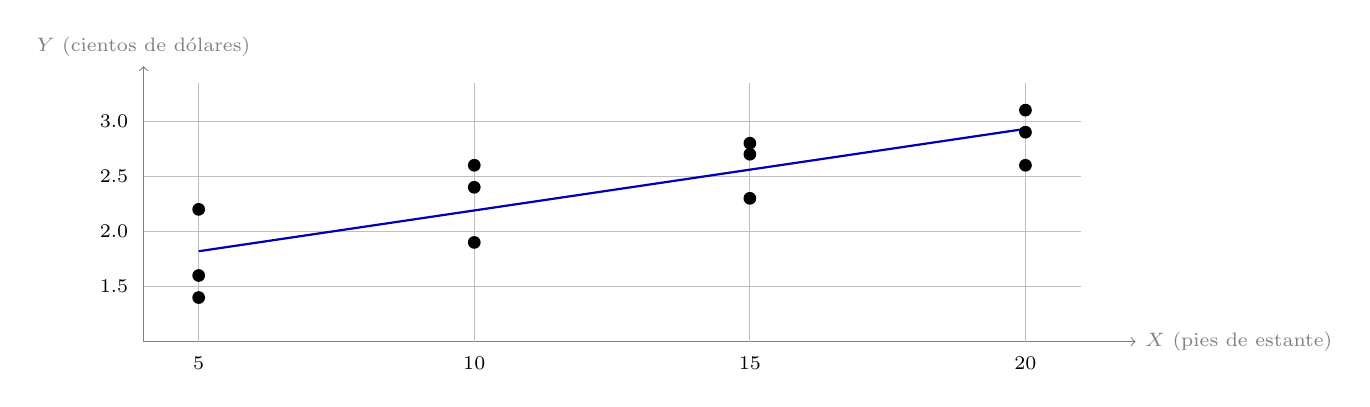
\begin{tikzpicture}[x=0.70cm,y=1.4cm,font=\scriptsize]
    \draw[->,gray] (4,1.0) -- (22,1.0) node[right] {$X$ (pies de estante)};
    \draw[->,gray] (4,1.0) -- (4,3.5) node[above] {$Y$ (cientos de dólares)};
    \foreach \x in {5,10,15,20} {
        \draw[gray!50] (\x,1.0) -- (\x,3.35);
        \node[below=2pt] at (\x,1.0) {\x};
    }
    \foreach \y in {1.5,2.0,2.5,3.0} {
        \draw[gray!50] (4,\y) -- (21,\y);
        \node[left=2pt] at (4,\y) {\y};
    }
    \draw[blue!70!black,thick] plot coordinates {(5,1.82) (20,2.93)};
    \foreach \x/\y in {5/1.6,5/2.2,5/1.4,10/1.9,10/2.4,10/2.6,15/2.3,15/2.7,15/2.8,20/2.6,20/2.9,20/3.1} {
        \fill[black] (\x,\y) circle (2.3pt);
    }
\end{tikzpicture}
    \caption{Diagrama de dispersión y recta estimada para el ejercicio 12.4.}
    \label{fig:clase4-petfood}
    \end{figure}
    \item[\textbf{b)}] La pendiente $0.074$ significa que un pie adicional de espacio de estante se asocia con un aumento medio estimado de $0.074$ cientos de dólares en ventas semanales, es decir, aproximadamente $7.40$ dólares.
    \item[\textbf{c)}] Para ocho pies,
    \[
    \widehat Y=1.45+0.074(8)=2.042\text{ cientos de dólares}.
    \]
    La venta media estimada es aproximadamente $\$204.20$ por semana.
\end{enumerate}

\subsection{Problema 5. Peso del correo y número de órdenes (ejercicio 12.7)}

Una empresa de ventas por correo quiere predecir el número de órdenes a partir del peso de los envíos recibidos. Se observaron 25 embarques. $X$ es el peso en libras y $Y$ el número de órdenes en miles.

\begin{table}[H]
\centering
\small
\begin{tabular}{r r@{\qquad\qquad}r r}
$X$ & $Y$ & $X$ & $Y$ \\ \hline
216 & 6.1 & 432 & 13.6 \\
283 & 9.1 & 409 & 12.8 \\
237 & 7.2 & 553 & 16.5 \\
203 & 7.5 & 572 & 17.1 \\
259 & 6.9 & 506 & 15.0 \\
374 & 11.5 & 528 & 16.2 \\
342 & 10.3 & 501 & 15.8 \\
301 & 9.5 & 628 & 19.0 \\
365 & 9.2 & 677 & 19.4 \\
384 & 10.6 & 602 & 19.1 \\
404 & 12.5 & 630 & 18.0 \\
426 & 12.9 & 652 & 20.2 \\
482 & 14.5 & & \\
\end{tabular}
\caption{Peso de los envíos y número de órdenes.}
\end{table}

Responda los siguientes incisos:
\begin{enumerate}
    \item[\textbf{a)}] Construya un diagrama de dispersión.
    \item[\textbf{b)}] Suponiendo una relación lineal, encuentre $b_0$ y $b_1$ por mínimos cuadrados.
    \item[\textbf{c)}] Interprete la pendiente.
    \item[\textbf{d)}] Prediga el número medio de órdenes para un envío de $500$ libras.
\end{enumerate}

\textbf{Solución.}
\begin{enumerate}
    \item[\textbf{a)}] El diagrama sugiere una asociación lineal positiva.
    \begin{figure}[H]
    \centering
    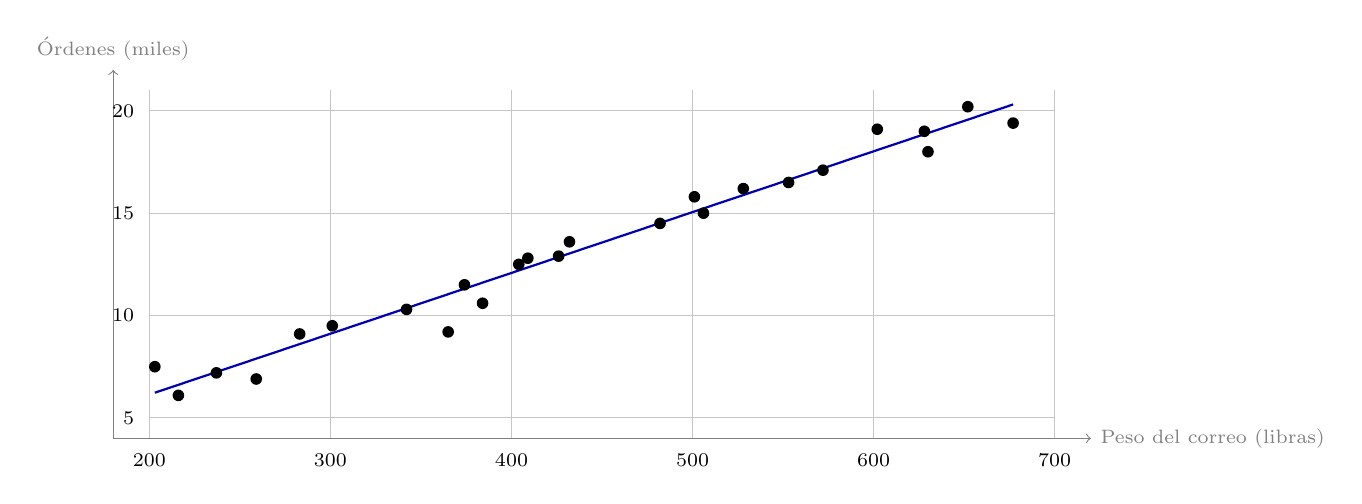
\begin{tikzpicture}[x=0.023cm,y=0.26cm,font=\scriptsize]
    \draw[->,gray] (180,4) -- (720,4) node[right] {Peso del correo (libras)};
    \draw[->,gray] (180,4) -- (180,22) node[above] {Órdenes (miles)};
    \foreach \x in {200,300,400,500,600,700} {
        \draw[gray!45] (\x,4) -- (\x,21);
        \node[below=2pt] at (\x,4) {\x};
    }
    \foreach \y in {5,10,15,20} {
        \draw[gray!45] (200,\y) -- (700,\y);
        \node[left=2pt] at (200,\y) {\y};
    }
    \draw[blue!70!black,thick] (203,6.23) -- (677,20.31);
    \foreach \x/\y in {216/6.1,283/9.1,237/7.2,203/7.5,259/6.9,374/11.5,342/10.3,301/9.5,365/9.2,384/10.6,404/12.5,426/12.9,482/14.5,432/13.6,409/12.8,553/16.5,572/17.1,506/15.0,528/16.2,501/15.8,628/19.0,677/19.4,602/19.1,630/18.0,652/20.2} {
        \fill[black] (\x,\y) circle (2.1pt);
    }
\end{tikzpicture}
    \caption{Diagrama de dispersión y recta estimada para el ejercicio 12.7.}
    \label{fig:clase4-mail}
    \end{figure}
    \item[\textbf{b)}] A partir de la tabla, las sumas necesarias son
    \[
    n=25,\quad \sum x_i=10966,\quad \sum y_i=330.5,\quad
    \sum x_i^2=5306182,\quad \sum x_iy_i=159704.7.
    \]
    Las sumas centradas son
    \begin{align*}
    C_{XX}&=\sum x_i^2-\frac{(\sum x_i)^2}{n}
    =5306182-\frac{10966^2}{25}=496055.76,\\
    C_{XY}&=\sum x_iy_i-\frac{(\sum x_i)(\sum y_i)}{n}
    =159704.7-\frac{(10966)(330.5)}{25}=14734.18.
    \end{align*}
    Por tanto,
    \begin{align*}
    b_1&=\frac{C_{XY}}{C_{XX}}\approx0.02970,\\
    b_0&=\bar y-b_1\bar x
    =13.22-(0.0297027)(438.64)\approx0.1912.
    \end{align*}
    La recta estimada es
    \[
    \widehat Y=0.1912+0.02970X.
    \]
    \item[\textbf{c)}] Como $Y$ está medido en miles de órdenes, la pendiente equivale a unas $0.02970$ miles, o $29.7$ órdenes adicionales en promedio por cada libra adicional recibida.
    \item[\textbf{d)}] Para $X=500$,
    \[
    \widehat Y=0.1912+0.0297027(500)\approx15.043\text{ miles de órdenes},
    \]
    es decir, aproximadamente $15043$ órdenes. Este valor está dentro del rango de pesos observado, de $203$ a $677$ libras.
\end{enumerate}

\subsection{Problema 6. Tamaño y renta de departamentos (ejercicio 12.9)}

Una agente inmobiliaria desea predecir la renta mensual a partir del tamaño de los departamentos de un vecindario. La muestra contiene 25 casos. En la tabla, $X$ es el tamaño en pies cuadrados y $Y$ la renta mensual en dólares.

\begin{table}[H]
\centering
\small
\begin{tabular}{r r@{\qquad\qquad}r r}
$X$ & $Y$ & $X$ & $Y$ \\ \hline
850 & 950 & 1369 & 1800 \\
1450 & 1600 & 1175 & 1400 \\
1085 & 1200 & 1225 & 1450 \\
1232 & 1500 & 1245 & 1100 \\
718 & 950 & 1259 & 1700 \\
1485 & 1700 & 1150 & 1200 \\
1136 & 1650 & 896 & 1150 \\
726 & 935 & 1361 & 1600 \\
700 & 875 & 1040 & 1650 \\
956 & 1150 & 755 & 1200 \\
1100 & 1400 & 1000 & 800 \\
1285 & 1650 & 1200 & 1750 \\
1985 & 2300 & & \\
\end{tabular}
\caption{Tamaño y renta mensual de los departamentos.}
\end{table}

Responda los siguientes incisos:
\begin{enumerate}
    \item[\textbf{a)}] Construya un diagrama de dispersión.
    \item[\textbf{b)}] Ajuste una recta por mínimos cuadrados.
    \item[\textbf{c)}] Interprete la pendiente.
    \item[\textbf{d)}] Estime la renta media para $1000$ pies cuadrados.
    \item[\textbf{e)}] Explique por qué no debe usarse la recta para predecir la renta de un departamento de $500$ pies cuadrados.
    \item[\textbf{f)}] Compare las opciones de $1000$ pies cuadrados por $\$1275$ y $1200$ pies cuadrados por $\$1425$. ¿Cuál recomendaría?
\end{enumerate}

\textbf{Solución.}
\begin{enumerate}
    \item[\textbf{a)}] El diagrama evidencia una tendencia positiva, aunque hay variabilidad considerable entre departamentos de tamaño parecido.
    \begin{figure}[H]
    \centering
    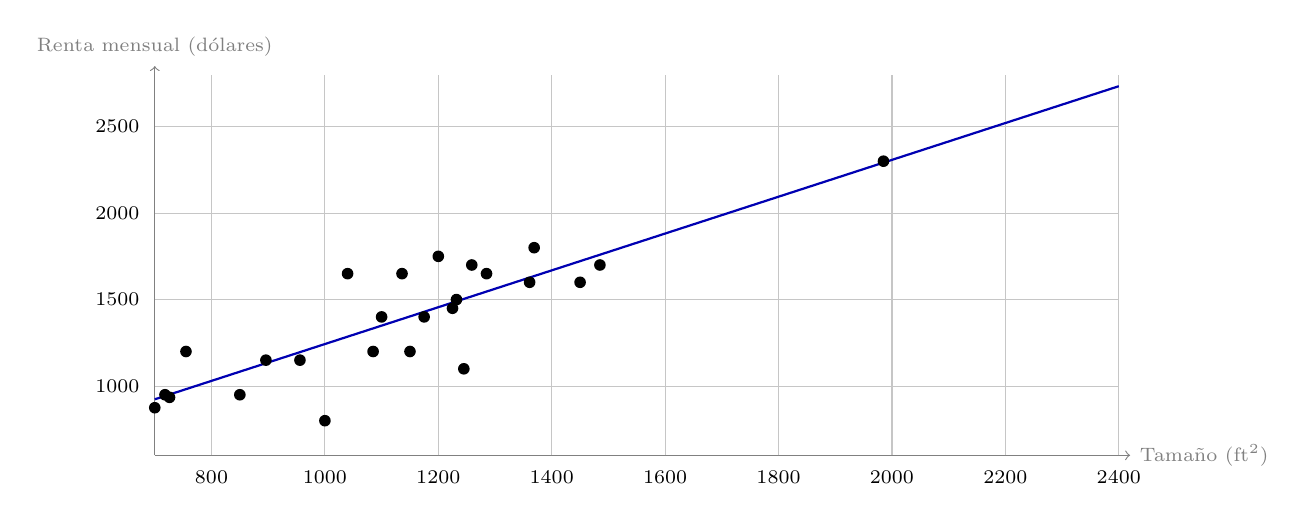
\begin{tikzpicture}[x=0.0072cm,y=0.0022cm,font=\scriptsize]
    \draw[->,gray] (700,600) -- (2420,600) node[right] {Tamaño ($\mathrm{ft}^2$)};
    \draw[->,gray] (700,600) -- (700,2850) node[above] {Renta mensual (dólares)};
    \foreach \x in {800,1000,1200,1400,1600,1800,2000,2200,2400} {
        \draw[gray!45] (\x,600) -- (\x,2800);
        \node[below=2pt] at (\x,600) {\x};
    }
    \foreach \y in {1000,1500,2000,2500} {
        \draw[gray!45] (700,\y) -- (2400,\y);
        \node[left=2pt] at (700,\y) {\y};
    }
    \draw[blue!70!black,thick] (700,923.7) -- (2400,2733.5);
    \foreach \x/\y in {850/950,1450/1600,1085/1200,1232/1500,718/950,1485/1700,1136/1650,726/935,700/875,956/1150,1100/1400,1285/1650,1985/2300,1369/1800,1175/1400,1225/1450,1245/1100,1259/1700,1150/1200,896/1150,1361/1600,1040/1650,755/1200,1000/800,1200/1750} {
        \fill[black] (\x,\y) circle (2.1pt);
    }
\end{tikzpicture}
    \caption{Diagrama de dispersión y recta estimada para el ejercicio 12.9.}
    \label{fig:clase4-rent}
    \end{figure}
    \item[\textbf{b)}] De la tabla se obtienen
    \[
    n=25,\quad \sum x_i=28383,\quad \sum y_i=34660,\quad
    \sum x_i^2=34223535,\quad \sum x_iy_i=41480210.
    \]
    Entonces,
    \begin{align*}
    C_{XX}&=34223535-\frac{28383^2}{25}=1999747.44,\\
    C_{XY}&=41480210-\frac{(28383)(34660)}{25}=2130018.8,
    \end{align*}
    y los coeficientes son
    \begin{align*}
    b_1&=\frac{2130018.8}{1999747.44}\approx1.06514,\\
    b_0&=\bar y-b_1\bar x
    =1386.4-(1.06514)(1135.32)\approx177.12.
    \end{align*}
    La ecuación estimada es
    \[
    \widehat Y=177.12+1.06514X.
    \]
    \item[\textbf{c)}] La pendiente indica que, según el ajuste, cada pie cuadrado adicional se asocia con un aumento medio de aproximadamente $\$1.07$ en la renta mensual.
    \item[\textbf{d)}] Para un departamento de $1000$ pies cuadrados,
    \[
    \widehat Y=177.12+1.06514(1000)\approx\$1242.26.
    \]
    \item[\textbf{e)}] Los tamaños de la muestra van de $700$ a $2300$ pies cuadrados. $500$ pies cuadrados queda fuera del rango observado, por lo que la predicción sería una extrapolación no respaldada por estos datos.
    \item[\textbf{f)}] La recta predice cerca de $\$1242.26$ para $1000$ pies cuadrados y $\$1455.29$ para $1200$ pies cuadrados. La primera renta ofrecida ($\$1275$) queda unos $\$32.74$ por encima de la predicción; la segunda ($\$1425$) queda unos $\$30.29$ por debajo. Si las demás condiciones son iguales, recomendaría la opción de $1200$ pies cuadrados, pues ofrece más espacio por un precio algo inferior al esperado según el modelo. Sin embargo, las diferencias son pequeñas frente a la variabilidad de las rentas; conviene considerar también el estado, la ubicación y otros atributos del inmueble.
\end{enumerate}

\section{Variación explicada y diagnóstico de residuos}

\subsection{Problema 7. Coeficiente de determinación (12.12)}

Responda los siguientes incisos:
\begin{enumerate}
    \item[\textbf{a)}] Calcule $SST$.
    \item[\textbf{b)}] Calcule el coeficiente de determinación $R^2$.
    \item[\textbf{c)}] Interprete el resultado.
\end{enumerate}

\textbf{Solución.}
\begin{enumerate}
    \item[\textbf{a)}] La variación total se descompone como $SST=SSR+SSE$, así que
    \[
    SST=36+4=40.
    \]
    \item[\textbf{b)}] Por definición,
    \[
    R^2=\frac{SSR}{SST}=\frac{36}{40}=0.90.
    \]
    \item[\textbf{c)}] El modelo explica el $90\%$ de la variación muestral de la respuesta alrededor de su media; el $10\%$ restante queda en los residuos. Esta descripción del ajuste no demuestra causalidad.
\end{enumerate}

\clearpage
\subsection{Problema 8. Patrón en los residuos a lo largo del tiempo (ejercicio 12.32)}

Los residuos observados para diez periodos consecutivos fueron los siguientes.

\begin{table}[H]
\centering
\begin{tabular}{r|r@{\qquad\qquad}r|r}
Periodo & Residuo & Periodo & Residuo \\ \hline
1 & $-5$ & 6 & $+1$ \\
2 & $-4$ & 7 & $+2$ \\
3 & $-3$ & 8 & $+3$ \\
4 & $-2$ & 9 & $+4$ \\
5 & $-1$ & 10 & $+5$ \\
\end{tabular}
\caption{Residuos por periodo del ejercicio 12.32.}
\end{table}

Responda los siguientes incisos:
\begin{enumerate}
    \item[\textbf{a)}] Represente los residuos en función del periodo y describa el patrón.
    \item[\textbf{b)}] Explique qué sugiere el patrón sobre la independencia de los errores.
\end{enumerate}

\textbf{Solución.}
\begin{enumerate}
    \item[\textbf{a)}] La gráfica muestra una tendencia creciente sostenida: los primeros residuos son negativos y luego se vuelven positivos, aumentando con el tiempo.
    \begin{figure}[H]
    \centering
    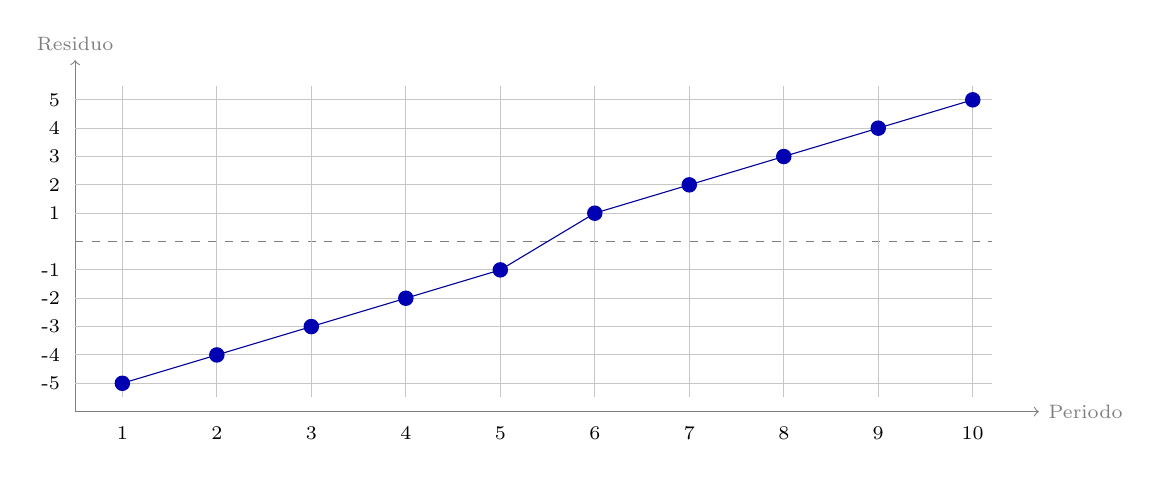
\begin{tikzpicture}[x=1.2cm,y=0.36cm,font=\scriptsize]
    \draw[->,gray] (0.5,-6) -- (10.7,-6) node[right] {Periodo};
    \draw[->,gray] (0.5,-6) -- (0.5,6.4) node[above] {Residuo};
    \draw[gray,dashed] (0.5,0) -- (10.2,0);
    \foreach \x in {1,2,3,4,5,6,7,8,9,10} {
        \draw[gray!45] (\x,-5.5) -- (\x,5.5);
        \node[below=2pt] at (\x,-6) {\x};
    }
    \foreach \y in {-5,-4,-3,-2,-1,1,2,3,4,5} {
        \draw[gray!45] (0.5,\y) -- (10.2,\y);
        \node[left=2pt] at (0.5,\y) {\y};
    }
    \draw[blue!60!black,thin] plot coordinates {(1,-5) (2,-4) (3,-3) (4,-2) (5,-1) (6,1) (7,2) (8,3) (9,4) (10,5)};
    \foreach \x/\e in {1/-5,2/-4,3/-3,4/-2,5/-1,6/1,7/2,8/3,9/4,10/5} {
        \fill[blue!70!black] (\x,\e) circle (2.8pt);
    }
\end{tikzpicture}
    \caption{Residuos del ejercicio 12.32 según el orden temporal.}
    \label{fig:clase4-residuos-tiempo}
    \end{figure}
    \item[\textbf{b)}] Los residuos no forman una nube aleatoria alrededor de cero. El patrón sugiere dependencia positiva entre periodos consecutivos, por lo que el supuesto de independencia de los errores es cuestionable. En un análisis real habría que investigar el orden temporal y la posible causa del patrón antes de confiar en la inferencia del modelo.
\end{enumerate}

\clearpage
\section{Ejercicio integrador final: análisis completo de los datos MAIL}

Este último ejercicio retoma los 25 embarques del problema 5 (ejercicio 12.7). La variable $X$ es el peso del correo recibido, en libras, y $Y$ es el número de órdenes, en miles. Se analizarán los datos con las herramientas descriptivas y de diagnóstico estudiadas en las clases de regresión. Las cantidades redondeadas en tablas pueden producir pequeñas diferencias respecto de los cálculos hechos con todos los decimales.

\subsection*{Enunciado}

Responda los siguientes incisos utilizando los 25 pares $(x_i,y_i)$ de la tabla del problema 5:
\begin{enumerate}
    \item[\textbf{a)}] Construya el diagrama de dispersión. Describa la dirección y la forma de la asociación, e indique los rangos observados de $X$ y $Y$.
    \item[\textbf{b)}] Calcule $n$, $\sum x_i$, $\sum y_i$, $\sum x_i^2$, $\sum y_i^2$ y $\sum x_iy_i$. Obtenga también $\bar x$ y $\bar y$.
    \item[\textbf{c)}] Calcule $C_{XX}$, $C_{YY}$ y $C_{XY}$. A partir de ellos, obtenga las varianzas, desviaciones estándar y covarianza muestrales de $X$ y $Y$.
    \item[\textbf{d)}] Encuentre la recta de mínimos cuadrados $\widehat Y=b_0+b_1X$, mostrando cómo obtiene la pendiente y la ordenada al origen.
    \item[\textbf{e)}] Interprete la pendiente y la ordenada al origen en el contexto del problema, teniendo en cuenta el rango observado de $X$.
    \item[\textbf{f)}] Calcule $\widehat y_i$ y $e_i=y_i-\widehat y_i$ para cada embarque. Presente los resultados en una tabla e identifique los residuos extremos.
    \item[\textbf{g)}] Compruebe las propiedades de los residuos de mínimos cuadrados con intercepto: $\sum e_i\approx0$, $\sum x_ie_i\approx0$ y $\sum\widehat y_i=\sum y_i$.
    \item[\textbf{h)}] Para el embarque 9, verifique $y_9-\bar y=(\widehat y_9-\bar y)+e_9$ y muestre esta descomposición gráficamente. Luego calcule $SST$, $SSR$ y $SSE$, verifique $SST=SSR+SSE$ y represente las tres cantidades.
    \item[\textbf{i)}] Calcule $R^2$ e interprete tanto la proporción explicada como la no explicada.
    \item[\textbf{j)}] Calcule el coeficiente de correlación de Pearson $r$ e interprete su signo e intensidad. Verifique que $R^2=r^2$.
    \item[\textbf{k)}] Calcule el promedio de cuadrados residuales $SSE/n$, su raíz cuadrada $\sqrt{SSE/n}$ y la estimación de la desviación estándar del error $s_e=\sqrt{SSE/(n-2)}$.
    \item[\textbf{l)}] Prediga la media del número de órdenes para un embarque de $500$ libras. Indique si se trata de interpolación o extrapolación y exprese la predicción en número de órdenes.
    \item[\textbf{m)}] Construya las gráficas de residuos contra valores ajustados y Q--Q. Úselas para discutir linealidad, igualdad de varianzas y normalidad. Comente qué se puede y qué no se puede concluir sobre independencia.
    \item[\textbf{n)}] Resuma si la recta parece útil para describir y predecir dentro del rango estudiado, y explique por qué los resultados no demuestran causalidad.
\end{enumerate}

\subsection*{Solución}

\begin{enumerate}
    \item[\textbf{a)}] El diagrama muestra una asociación creciente y aproximadamente lineal: embarques más pesados tienden a corresponder a un mayor número de órdenes. El peso varía entre $203$ y $677$ libras, y las órdenes entre $6.1$ y $20.2$ miles. Los trazos verticales muestran las diferencias entre cada respuesta observada y la recta ajustada; el punto rojo señala la predicción para $X=500$.
    \begin{figure}[H]
    \centering
    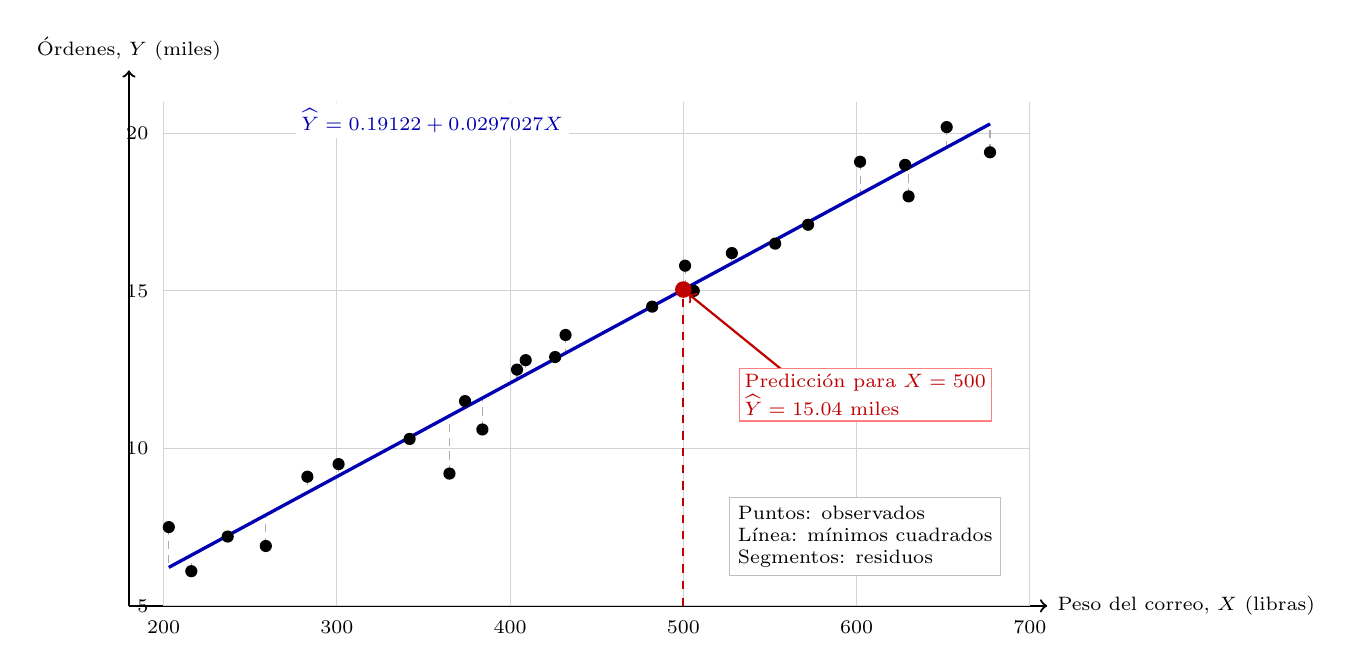
\begin{tikzpicture}[x=0.022cm,y=0.40cm,font=\scriptsize]
    \draw[->,thick] (180,5) -- (710,5) node[right] {Peso del correo, $X$ (libras)};
    \draw[->,thick] (180,5) -- (180,22) node[above] {Órdenes, $Y$ (miles)};
    \foreach \xx in {200,300,400,500,600,700} {
        \draw[gray!35] (\xx,5) -- (\xx,21);
        \node[below=2pt] at (\xx,5) {\xx};
    }
    \foreach \yy in {5,10,15,20} {
        \draw[gray!35] (200,\yy) -- (700,\yy);
        \node[left=2pt] at (200,\yy) {\yy};
    }
    \draw[gray!65,densely dashed] (216,6.1000) -- (216,6.6070);
    \draw[gray!65,densely dashed] (283,9.1000) -- (283,8.5971);
    \draw[gray!65,densely dashed] (237,7.2000) -- (237,7.2308);
    \draw[gray!65,densely dashed] (203,7.5000) -- (203,6.2209);
    \draw[gray!65,densely dashed] (259,6.9000) -- (259,7.8842);
    \draw[gray!65,densely dashed] (374,11.5000) -- (374,11.3000);
    \draw[gray!65,densely dashed] (342,10.3000) -- (342,10.3495);
    \draw[gray!65,densely dashed] (301,9.5000) -- (301,9.1317);
    \draw[gray!65,densely dashed] (365,9.2000) -- (365,11.0327);
    \draw[gray!65,densely dashed] (384,10.6000) -- (384,11.5970);
    \draw[gray!65,densely dashed] (404,12.5000) -- (404,12.1911);
    \draw[gray!65,densely dashed] (426,12.9000) -- (426,12.8446);
    \draw[gray!65,densely dashed] (482,14.5000) -- (482,14.5079);
    \draw[gray!65,densely dashed] (432,13.6000) -- (432,13.0228);
    \draw[gray!65,densely dashed] (409,12.8000) -- (409,12.3396);
    \draw[gray!65,densely dashed] (553,16.5000) -- (553,16.6168);
    \draw[gray!65,densely dashed] (572,17.1000) -- (572,17.1811);
    \draw[gray!65,densely dashed] (506,15.0000) -- (506,15.2208);
    \draw[gray!65,densely dashed] (528,16.2000) -- (528,15.8742);
    \draw[gray!65,densely dashed] (501,15.8000) -- (501,15.0723);
    \draw[gray!65,densely dashed] (628,19.0000) -- (628,18.8445);
    \draw[gray!65,densely dashed] (677,19.4000) -- (677,20.2999);
    \draw[gray!65,densely dashed] (602,19.1000) -- (602,18.0722);
    \draw[gray!65,densely dashed] (630,18.0000) -- (630,18.9039);
    \draw[gray!65,densely dashed] (652,20.2000) -- (652,19.5574);
    \draw[blue!70!black,very thick] (203,6.2209) -- (677,20.2999);
    \fill[black] (216,6.1) circle (2.2pt);
    \fill[black] (283,9.1) circle (2.2pt);
    \fill[black] (237,7.2) circle (2.2pt);
    \fill[black] (203,7.5) circle (2.2pt);
    \fill[black] (259,6.9) circle (2.2pt);
    \fill[black] (374,11.5) circle (2.2pt);
    \fill[black] (342,10.3) circle (2.2pt);
    \fill[black] (301,9.5) circle (2.2pt);
    \fill[black] (365,9.2) circle (2.2pt);
    \fill[black] (384,10.6) circle (2.2pt);
    \fill[black] (404,12.5) circle (2.2pt);
    \fill[black] (426,12.9) circle (2.2pt);
    \fill[black] (482,14.5) circle (2.2pt);
    \fill[black] (432,13.6) circle (2.2pt);
    \fill[black] (409,12.8) circle (2.2pt);
    \fill[black] (553,16.5) circle (2.2pt);
    \fill[black] (572,17.1) circle (2.2pt);
    \fill[black] (506,15.0) circle (2.2pt);
    \fill[black] (528,16.2) circle (2.2pt);
    \fill[black] (501,15.8) circle (2.2pt);
    \fill[black] (628,19.0) circle (2.2pt);
    \fill[black] (677,19.4) circle (2.2pt);
    \fill[black] (602,19.1) circle (2.2pt);
    \fill[black] (630,18.0) circle (2.2pt);
    \fill[black] (652,20.2) circle (2.2pt);
    \draw[red!75!black,dashed,thick] (500,5) -- (500,15.0426);
    \fill[red!75!black] (500,15.0426) circle (3pt);
    \draw[red!75!black,->,thick] (577,11.6) -- (503,14.9);
    \node[red!75!black,align=left,draw=red!50,fill=white,inner sep=2pt] at (605,11.7)
        {Predicción para $X=500$\\$\widehat Y=15.04$ miles};
    \node[blue!70!black,fill=white,inner sep=2pt] at (355,20.4) {$\widehat Y=0.19122+0.0297027X$};
    \node[align=left,draw=gray!50,fill=white,inner sep=3pt] at (605,7.2)
        {Puntos: observados\\Línea: mínimos cuadrados\\Segmentos: residuos};
\end{tikzpicture}
    \caption{Datos MAIL, recta de mínimos cuadrados, residuos verticales y predicción en $X=500$.}
    \label{fig:clase4-mail-integrador-dispersion}
    \end{figure}

    \item[\textbf{b)}] Hay $n=25$ observaciones. Al sumar los datos de la tabla del problema 5 se obtiene
    \begin{align*}
    \sum x_i&=10966,& \sum y_i&=330.5,\\
    \sum x_i^2&=5306182,& \sum y_i^2&=4818.97,\\
    \sum x_iy_i&=159704.7.
    \end{align*}
    Así,
    \[
    \bar x=\frac{10966}{25}=438.64\text{ libras},\qquad
    \bar y=\frac{330.5}{25}=13.22\text{ miles de órdenes}.
    \]

    \item[\textbf{c)}] Las sumas centradas se calculan restando el efecto de las medias:
    \begin{align*}
    C_{XX}&=\sum x_i^2-\frac{(\sum x_i)^2}{n}
    =5306182-\frac{10966^2}{25}=496055.76,\\
    C_{YY}&=\sum y_i^2-\frac{(\sum y_i)^2}{n}
    =4818.97-\frac{330.5^2}{25}=449.76,\\
    C_{XY}&=\sum x_iy_i-\frac{(\sum x_i)(\sum y_i)}{n}
    =159704.7-\frac{(10966)(330.5)}{25}=14734.18.
    \end{align*}
    Con denominador $n-1=24$, las medidas muestrales son
    \begin{align*}
    s_X^2&=\frac{C_{XX}}{24}=20668.99\text{ libras}^2,&
    s_X&=\sqrt{20668.99}\approx143.77\text{ libras},\\
    s_Y^2&=\frac{C_{YY}}{24}=18.74\text{ (miles de órdenes)}^2,&
    s_Y&=\sqrt{18.74}\approx4.329\text{ miles de órdenes},\\
    s_{XY}&=\frac{C_{XY}}{24}\approx613.9242\text{ libras}\cdot\text{miles de órdenes}.
    \end{align*}
    La covarianza es positiva. Si se emplea denominador $n$ en covarianza y varianzas, sus valores cambian, pero su cociente para calcular la pendiente no cambia.

    \item[\textbf{d)}] La pendiente y la ordenada al origen son
    \begin{align*}
    b_1&=\frac{C_{XY}}{C_{XX}}=\frac{14734.18}{496055.76}\approx0.0297027,\\
    b_0&=\bar y-b_1\bar x
    =13.22-(0.0297027)(438.64)\approx0.19122.
    \end{align*}
    Por tanto, la recta estimada es
    \[
    \boxed{\widehat Y=0.19122+0.0297027X}.
    \]

    \item[\textbf{e)}] La pendiente indica que, dentro del rango estudiado, cada libra adicional de correo se asocia con un aumento medio estimado de $0.02970$ miles de órdenes, es decir, aproximadamente $29.7$ órdenes. La ordenada al origen predice $0.191$ miles de órdenes para $X=0$, pero cero libras está muy fuera del rango observado; por ello esa ordenada es necesaria para definir la recta, pero su interpretación operativa aquí no es confiable.

    \item[\textbf{f)}] Para cada observación se usa $\widehat y_i=0.1912213+0.02970267x_i$ y luego $e_i=y_i-\widehat y_i$. Por ejemplo, en el primer embarque,
    \[
    \widehat y_1=0.1912213+0.02970267(216)\approx6.6070,\qquad
    e_1=6.1-6.6070\approx-0.5070.
    \]
    La tabla presenta las predicciones, los residuos y sus cuadrados; todas las cantidades de respuesta están en miles de órdenes.
    \begin{table}[H]
    \centering
    \small
    \setlength{\tabcolsep}{5pt}
    \renewcommand{\arraystretch}{1.04}
    \begin{tabular}{r r r r r r}
    \hline
    $i$ & $x_i$ & $y_i$ & $\widehat y_i$ & $e_i$ & $e_i^2$ \\
    \hline
    1 & 216 & 6.1 & 6.6070 & -0.5070 & 0.2570 \\
2 & 283 & 9.1 & 8.5971 & 0.5029 & 0.2529 \\
3 & 237 & 7.2 & 7.2308 & -0.0308 & 0.0009 \\
4 & 203 & 7.5 & 6.2209 & 1.2791 & 1.6362 \\
5 & 259 & 6.9 & 7.8842 & -0.9842 & 0.9687 \\
6 & 374 & 11.5 & 11.3000 & 0.2000 & 0.0400 \\
7 & 342 & 10.3 & 10.3495 & -0.0495 & 0.0025 \\
8 & 301 & 9.5 & 9.1317 & 0.3683 & 0.1356 \\
9 & 365 & 9.2 & 11.0327 & -1.8327 & 3.3588 \\
10 & 384 & 10.6 & 11.5970 & -0.9970 & 0.9941 \\
11 & 404 & 12.5 & 12.1911 & 0.3089 & 0.0954 \\
12 & 426 & 12.9 & 12.8446 & 0.0554 & 0.0031 \\
13 & 482 & 14.5 & 14.5079 & -0.0079 & 0.0001 \\
14 & 432 & 13.6 & 13.0228 & 0.5772 & 0.3332 \\
15 & 409 & 12.8 & 12.3396 & 0.4604 & 0.2120 \\
16 & 553 & 16.5 & 16.6168 & -0.1168 & 0.0136 \\
17 & 572 & 17.1 & 17.1811 & -0.0811 & 0.0066 \\
18 & 506 & 15.0 & 15.2208 & -0.2208 & 0.0487 \\
19 & 528 & 16.2 & 15.8742 & 0.3258 & 0.1061 \\
20 & 501 & 15.8 & 15.0723 & 0.7277 & 0.5296 \\
21 & 628 & 19.0 & 18.8445 & 0.1555 & 0.0242 \\
22 & 677 & 19.4 & 20.2999 & -0.8999 & 0.8099 \\
23 & 602 & 19.1 & 18.0722 & 1.0278 & 1.0563 \\
24 & 630 & 18.0 & 18.9039 & -0.9039 & 0.8170 \\
25 & 652 & 20.2 & 19.5574 & 0.6426 & 0.4130 \\
    \hline
    \end{tabular}
    \caption{Valores ajustados y residuos para los 25 embarques MAIL.}
    \label{tab:clase4-mail-residuos-integrador}
    \end{table}
    Los residuos de mayor magnitud son los de las observaciones 9 ($e_9\approx-1.8327$), 4 ($e_4\approx1.2791$) y 23 ($e_{23}\approx1.0278$) miles de órdenes. Conviene identificarlos al revisar el ajuste, sin clasificarlos automáticamente como errores o valores atípicos.

    \item[\textbf{g)}] Con los valores calculados sin redondear se verifica que
    \[
    \sum_{i=1}^{25}e_i\approx0,\qquad
    \sum_{i=1}^{25}x_ie_i\approx0,\qquad
    \sum_{i=1}^{25}\widehat y_i=\sum_{i=1}^{25}y_i=330.5.
    \]
    Las pequeñas diferencias que se obtengan al sumar la tabla se deben al redondeo. La suma residual nula se sigue del ajuste por mínimos cuadrados con intercepto; la segunda igualdad expresa que los residuos no conservan una tendencia lineal con $X$ en el ajuste.

    \item[\textbf{h)}] Para el embarque 9, $y_9=9.2$, $\widehat y_9\approx11.0327$ y $\bar y=13.22$. Por tanto,
    \[
    y_9-\bar y=-4.02=(\widehat y_9-\bar y)+e_9
    \approx-2.1873+(-1.8327).
    \]
    La figura distingue la desviación total respecto de la media, su parte asociada con el ajuste y el residuo de esta observación.
    \begin{figure}[H]
    \centering
    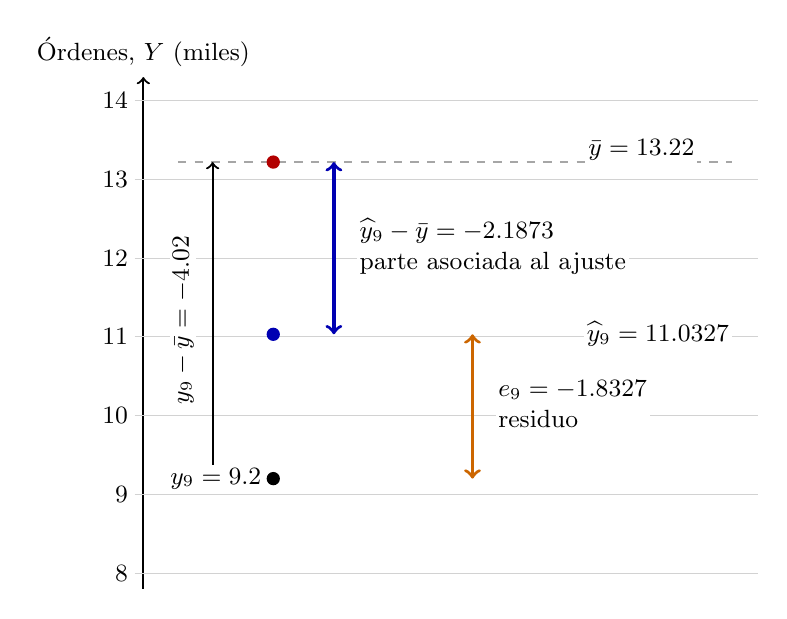
\begin{tikzpicture}[x=2.2cm,y=1cm,font=\small]
    \draw[->,thick] (-0.75,7.8) -- (-0.75,14.3) node[above] {Órdenes, $Y$ (miles)};
    \foreach \yy in {8,9,10,11,12,13,14} {
        \draw[gray!35] (-0.8,\yy) -- (2.8,\yy);
        \node[left=2pt] at (-0.75,\yy) {\yy};
    }
    \draw[gray!70,dashed,thick] (-0.55,13.22) -- (2.65,13.22);
    \node[anchor=west,fill=white,inner sep=1pt] at (1.8,13.38) {$\bar y=13.22$};
    \draw[black,<->,thick] (-0.35,9.2) -- (-0.35,13.22);
    \node[rotate=90,fill=white,inner sep=1pt] at (-0.52,11.21) {$y_9-\bar y=-4.02$};
    \draw[blue!70!black,<->,very thick] (0.35,11.0327) -- (0.35,13.22);
    \node[anchor=west,align=left,fill=white,inner sep=1pt] at (0.48,12.15) {$\widehat y_9-\bar y=-2.1873$\\parte asociada al ajuste};
    \draw[orange!80!black,<->,very thick] (1.15,9.2) -- (1.15,11.0327);
    \node[anchor=west,align=left,fill=white,inner sep=1pt] at (1.28,10.15) {$e_9=-1.8327$\\residuo};
    \fill[black] (0,9.2) circle (2.4pt);
    \fill[blue!70!black] (0,11.0327) circle (2.4pt);
    \fill[red!70!black] (0,13.22) circle (2.4pt);
    \node[anchor=east,fill=white,inner sep=1pt] at (-0.05,9.2) {$y_9=9.2$};
    \node[anchor=east,fill=white,inner sep=1pt] at (2.65,11.0327) {$\widehat y_9=11.0327$};
\end{tikzpicture}
    \caption{Descomposición de la desviación de $y_9$ respecto de su media.}
    \label{fig:clase4-mail-integrador-descomposicion}
    \end{figure}
    La variación total de las órdenes respecto de su media es
    \[
    SST=C_{YY}=449.76.
    \]
    La parte explicada por la recta y la parte residual son
    \begin{align*}
    SSR&=b_1^2C_{XX}=\frac{C_{XY}^2}{C_{XX}}=b_1C_{XY}\approx437.6445,\\
    SSE&=\sum e_i^2\approx12.1155.
    \end{align*}
    Se comprueba la descomposición
    \[
    SST=SSR+SSE\approx437.6445+12.1155=449.7600.
    \]
    La figura permite comparar visualmente las partes explicada y residual de la variación.
    \begin{figure}[H]
    \centering
    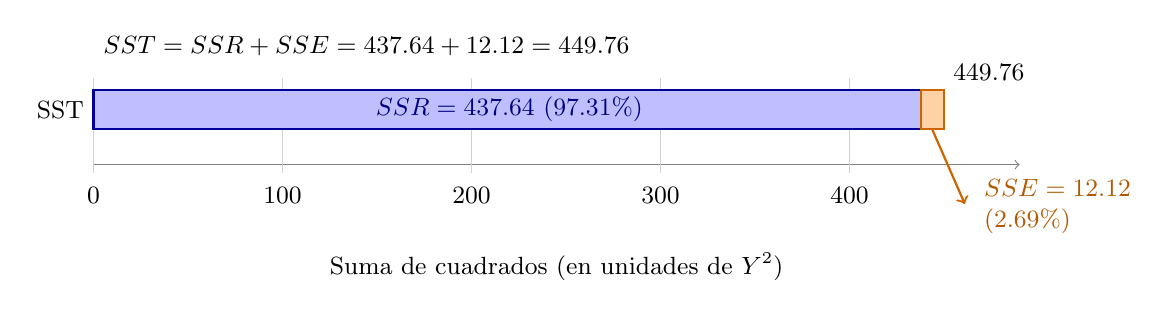
\begin{tikzpicture}[x=0.024cm,y=1cm,font=\small]
    \draw[->,gray] (0,0.55) -- (490,0.55);
    \node[anchor=west] at (0,2.05) {$SST=SSR+SSE=437.64+12.12=449.76$};
    \foreach \xx in {0,100,200,300,400} {
        \draw[gray!35] (\xx,0.45) -- (\xx,1.65);
        \node[below=2pt] at (\xx,0.45) {\xx};
    }
    \node[left,align=right] at (0,1.25) {SST};
    \draw[blue!60!black,thick,fill=blue!25] (0,1) rectangle (437.6445,1.5);
    \draw[orange!80!black,thick,fill=orange!35] (437.6445,1) rectangle (449.7600,1.5);
    \node[blue!50!black] at (220,1.25) {$SSR=437.64$ (97.31\%)};
    \draw[orange!80!black,->,thick] (443.7,1) -- (461,0.05);
    \node[orange!70!black,align=left,anchor=west] at (466,0.02) {$SSE=12.12$\\(2.69\%)};
    \node[above right] at (449.76,1.5) {$449.76$};
    \node[below] at (245,-0.45) {Suma de cuadrados (en unidades de $Y^2$)};
\end{tikzpicture}
    \caption{Descomposición de la variación total en variación explicada y residual.}
    \label{fig:clase4-mail-integrador-variacion}
    \end{figure}

    \item[\textbf{i)}] El coeficiente de determinación es
    \[
    R^2=\frac{SSR}{SST}=\frac{437.6445}{449.76}\approx0.97306.
    \]
    La recta explica aproximadamente el $97.31\%$ de la variación muestral del número de órdenes; cerca del $2.69\%$ queda en los residuos. Esto describe el ajuste de esta muestra y no garantiza por sí solo predicciones precisas en cualquier situación.

    \item[\textbf{j)}] El coeficiente de correlación es
    \[
    r=\frac{C_{XY}}{\sqrt{C_{XX}C_{YY}}}
    =\frac{14734.18}{\sqrt{(496055.76)(449.76)}}\approx0.98644.
    \]
    Es positivo, como la pendiente, y cercano a uno: en estos datos hay una asociación lineal positiva muy marcada. Además,
    \[
    r^2\approx(0.98644)^2\approx0.97306=R^2,
    \]
    de acuerdo con la relación entre correlación y determinación en regresión simple con intercepto.

    \item[\textbf{k)}] La dispersión cuadrática descriptiva por observación es
    \[
    \frac{SSE}{n}=\frac{12.1155}{25}\approx0.48462\text{ (miles de órdenes)}^2,
    \]
    y su raíz cuadrada, la raíz del promedio cuadrático residual en las unidades de $Y$, es
    \[
    \sqrt{\frac{SSE}{n}}\approx0.6961\text{ miles de órdenes}.
    \]
    Para estimar la desviación estándar del error en el modelo se usa el denominador $n-2$, por los dos coeficientes estimados:
    \[
    s_e=\sqrt{\frac{SSE}{n-2}}=\sqrt{\frac{12.1155}{23}}\approx0.7258\text{ miles de órdenes},
    \]
    cerca de $726$ órdenes. Esta medida resume el tamaño típico de las desviaciones alrededor de la recta; no es un intervalo de predicción.

    \item[\textbf{l)}] Para $X=500$ libras, que está dentro del intervalo observado $[203,677]$, la predicción es una interpolación:
    \[
    \widehat Y=0.1912213+0.02970267(500)\approx15.0426\text{ miles de órdenes}.
    \]
    El modelo estima una media de aproximadamente $15.04$ miles, o $15043$ órdenes. Se trata de una media estimada, no del conteo exacto que necesariamente tendrá un embarque particular.

    \item[\textbf{m)}] Al revisar LINI, la nube respalda aproximadamente la linealidad; en residuos contra valores ajustados no aparece una curva o un embudo pronunciado; la dispersión parece aproximadamente centrada en cero, aunque hay algunos residuos más alejados, ya señalados en el inciso f). En el gráfico Q--Q, la mayoría de los puntos sigue una tendencia aproximadamente lineal, con desviaciones en las colas. Con 25 datos estos gráficos no prueban normalidad ni varianza constante; solo muestran si los supuestos parecen razonables.
    \begin{figure}[H]
    \centering
    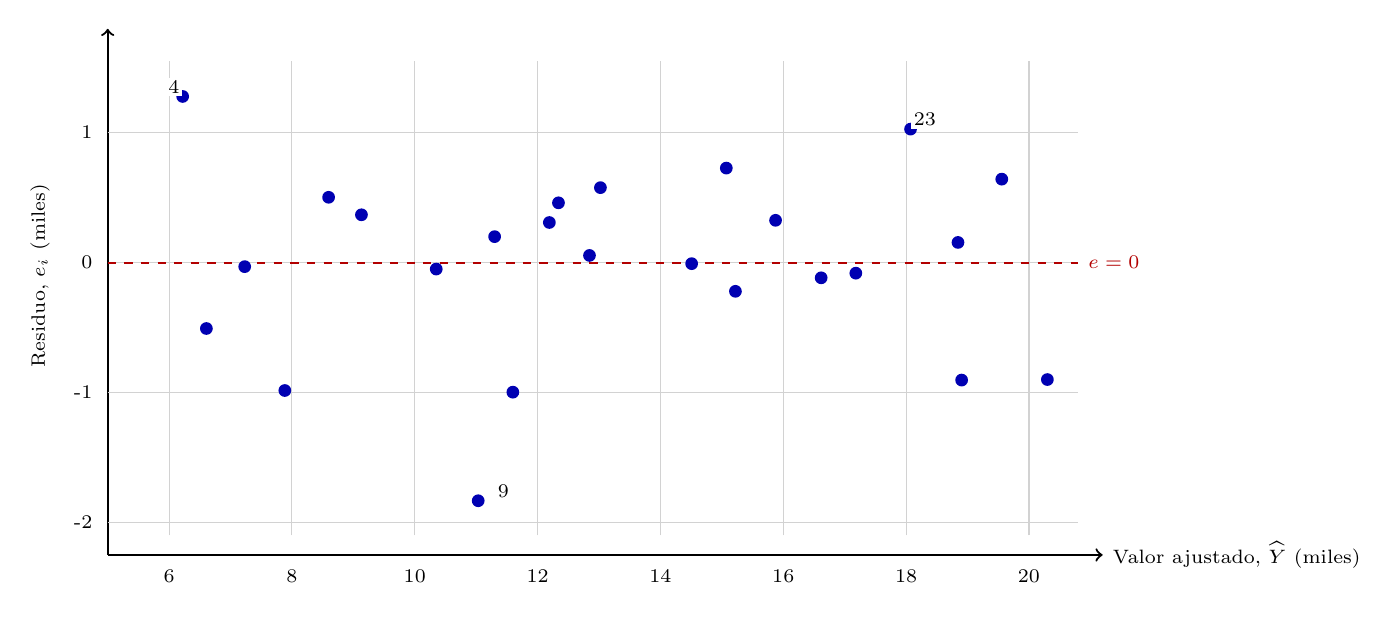
\begin{tikzpicture}[x=0.78cm,y=1.65cm,font=\scriptsize]
    \draw[->,thick] (5,-2.25) -- (21.2,-2.25) node[right] {Valor ajustado, $\widehat Y$ (miles)};
    \draw[->,thick] (5,-2.25) -- (5,1.8);
    \foreach \xx in {6,8,10,12,14,16,18,20} {
        \draw[gray!35] (\xx,-2.1) -- (\xx,1.55);
        \node[below=2pt] at (\xx,-2.25) {\xx};
    }
    \foreach \yy in {-2,-1,0,1} {
        \draw[gray!35] (5,\yy) -- (20.8,\yy);
        \node[left=2pt] at (5,\yy) {\yy};
    }
    \draw[red!70!black,dashed,thick] (5,0) -- (20.8,0) node[right] {$e=0$};
    \fill[blue!70!black] (6.6070,-0.5070) circle (2.3pt);
    \fill[blue!70!black] (8.5971,0.5029) circle (2.3pt);
    \fill[blue!70!black] (7.2308,-0.0308) circle (2.3pt);
    \fill[blue!70!black] (6.2209,1.2791) circle (2.3pt);
    \fill[blue!70!black] (7.8842,-0.9842) circle (2.3pt);
    \fill[blue!70!black] (11.3000,0.2000) circle (2.3pt);
    \fill[blue!70!black] (10.3495,-0.0495) circle (2.3pt);
    \fill[blue!70!black] (9.1317,0.3683) circle (2.3pt);
    \fill[blue!70!black] (11.0327,-1.8327) circle (2.3pt);
    \fill[blue!70!black] (11.5970,-0.9970) circle (2.3pt);
    \fill[blue!70!black] (12.1911,0.3089) circle (2.3pt);
    \fill[blue!70!black] (12.8446,0.0554) circle (2.3pt);
    \fill[blue!70!black] (14.5079,-0.0079) circle (2.3pt);
    \fill[blue!70!black] (13.0228,0.5772) circle (2.3pt);
    \fill[blue!70!black] (12.3396,0.4604) circle (2.3pt);
    \fill[blue!70!black] (16.6168,-0.1168) circle (2.3pt);
    \fill[blue!70!black] (17.1811,-0.0811) circle (2.3pt);
    \fill[blue!70!black] (15.2208,-0.2208) circle (2.3pt);
    \fill[blue!70!black] (15.8742,0.3258) circle (2.3pt);
    \fill[blue!70!black] (15.0723,0.7277) circle (2.3pt);
    \fill[blue!70!black] (18.8445,0.1555) circle (2.3pt);
    \fill[blue!70!black] (20.2999,-0.8999) circle (2.3pt);
    \fill[blue!70!black] (18.0722,1.0278) circle (2.3pt);
    \fill[blue!70!black] (18.9039,-0.9039) circle (2.3pt);
    \fill[blue!70!black] (19.5574,0.6426) circle (2.3pt);
    \node[above right,fill=white,inner sep=1pt] at (11.3000,-1.8327) {9};
    \node[above left,fill=white,inner sep=1pt] at (6.2209,1.2791) {4};
    \node[above right,fill=white,inner sep=1pt] at (18.0722,1.0278) {23};
    \node[rotate=90,fill=white,inner sep=1pt] at (3.9,-0.1) {Residuo, $e_i$ (miles)};
\end{tikzpicture}
    \caption{Residuos contra valores ajustados para examinar forma y dispersión. Se etiquetan tres residuos de mayor magnitud.}
    \label{fig:clase4-mail-integrador-residuos}
    \end{figure}
    \begin{figure}[H]
    \centering
    \begin{tikzpicture}[x=2.7cm,y=2.4cm,font=\scriptsize]
    \draw[->,thick] (-2.2,-2.15) -- (2.25,-2.15) node[right] {Cuantil normal teórico};
    \draw[->,thick] (-2.2,-2.15) -- (-2.2,1.75);
    \foreach \xx in {-2,-1,0,1,2} {
        \draw[gray!35] (\xx,-2.05) -- (\xx,1.55);
        \node[below=2pt] at (\xx,-2.15) {\xx};
    }
    \foreach \yy in {-2,-1,0,1} {
        \draw[gray!35] (-2.1,\yy) -- (2.1,\yy);
        \node[left=2pt] at (-2.2,\yy) {\yy};
    }
    \draw[red!70!black,dashed,thick] (-2.05,-1.489) -- (2.05,1.489);
    \fill[blue!70!black] (-1.9642,-1.8327) circle (2.3pt);
    \fill[blue!70!black] (-1.5192,-0.9970) circle (2.3pt);
    \fill[blue!70!black] (-1.2593,-0.9842) circle (2.3pt);
    \fill[blue!70!black] (-1.0644,-0.9039) circle (2.3pt);
    \fill[blue!70!black] (-0.9034,-0.8999) circle (2.3pt);
    \fill[blue!70!black] (-0.7629,-0.5070) circle (2.3pt);
    \fill[blue!70!black] (-0.6360,-0.2208) circle (2.3pt);
    \fill[blue!70!black] (-0.5187,-0.1168) circle (2.3pt);
    \fill[blue!70!black] (-0.4081,-0.0811) circle (2.3pt);
    \fill[blue!70!black] (-0.3024,-0.0495) circle (2.3pt);
    \fill[blue!70!black] (-0.1999,-0.0308) circle (2.3pt);
    \fill[blue!70!black] (-0.0994,-0.0079) circle (2.3pt);
    \fill[blue!70!black] (0.0000,0.0554) circle (2.3pt);
    \fill[blue!70!black] (0.0994,0.1555) circle (2.3pt);
    \fill[blue!70!black] (0.1999,0.2000) circle (2.3pt);
    \fill[blue!70!black] (0.3024,0.3089) circle (2.3pt);
    \fill[blue!70!black] (0.4081,0.3258) circle (2.3pt);
    \fill[blue!70!black] (0.5187,0.3683) circle (2.3pt);
    \fill[blue!70!black] (0.6360,0.4604) circle (2.3pt);
    \fill[blue!70!black] (0.7629,0.5029) circle (2.3pt);
    \fill[blue!70!black] (0.9034,0.5772) circle (2.3pt);
    \fill[blue!70!black] (1.0644,0.6426) circle (2.3pt);
    \fill[blue!70!black] (1.2593,0.7277) circle (2.3pt);
    \fill[blue!70!black] (1.5192,1.0278) circle (2.3pt);
    \fill[blue!70!black] (1.9642,1.2791) circle (2.3pt);
    \node[rotate=90,fill=white,inner sep=1pt] at (-2.35,-0.2) {Residuos ordenados (miles)};
\end{tikzpicture}
    \caption{Gráfico Q--Q de los residuos con cuantiles normales teóricos aproximados.}
    \label{fig:clase4-mail-integrador-qq}
    \end{figure}
    La independencia no puede diagnosticarse con el orden en que los pares aparecen en la tabla, pues ese orden no representa una secuencia temporal o un diseño ordenado. Debe justificarse con la forma en que se seleccionaron los embarques y con conocimiento del proceso.

    \item[\textbf{n)}] La nube, la pendiente, la correlación y los residuos respaldan el uso descriptivo de una recta para estos datos y predicciones dentro del rango observado. Sin embargo, ni una correlación alta ni un $R^2$ alto demuestran que el peso del correo cause el número de órdenes: campañas, temporada u otros factores podrían influir en ambas variables.
\end{enumerate}